% 第 17 题四棱锥 P-ABCD：按固定源 PDF 的顶点相对位置重绘；虚线仅 DA、AC 两条。
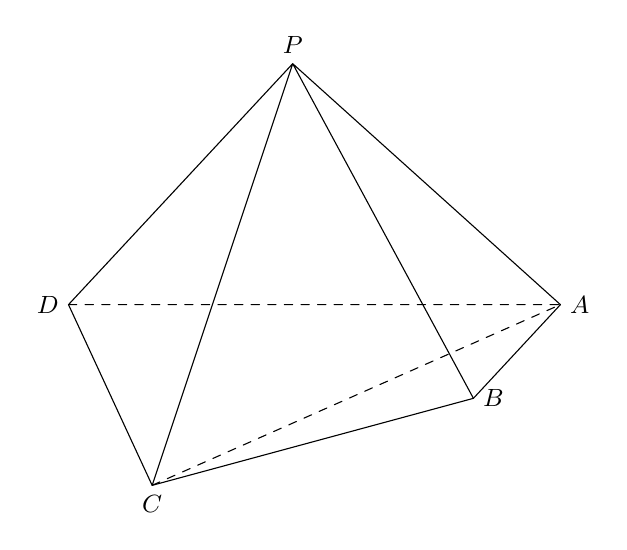
\begin{tikzpicture}[line cap=round,line join=round,font=\small,scale=0.85]
\coordinate (P) at (2.1,6.3);
\coordinate (D) at (-1.25,2.7);
\coordinate (A) at (6.1,2.7);
\coordinate (B) at (4.8,1.3);
\coordinate (C) at (0,0);
\draw (P)--(D) (P)--(A) (P)--(B) (P)--(C);
\draw (D)--(C) (C)--(B) (B)--(A);
\draw[dashed] (D)--(A) (C)--(A);
\node[above] at (P) {$P$};
\node[left] at (D) {$D$};
\node[right] at (A) {$A$};
\node[right] at (B) {$B$};
\node[below] at (C) {$C$};
\end{tikzpicture}
